\begin{exercises} 
\item Consider the basic functions $f(x) = x^3$ and $g(x) = \sin(x)$.
\ba
	\item Let $h(x) = f(g(x))$.  Find the exact instantaneous rate of change of $h$ at the point where $x = \frac{\pi}{4}.$
	\item Which function is changing most rapidly at $x = 0.25$:  $h(x) = f(g(x))$ or $r(x) = g(f(x))$?  Why?
	\item Let $h(x) = f(g(x))$ and $r(x) = g(f(x))$.  Which of these functions has a derivative that is periodic?  Why?
\ea
\item Let $u(x)$ be a differentiable function.  For each of the following functions, determine the derivative.  Each response will involve $u$ and/or $u'$.
\ba
	\item $p(x) = e^{u(x)}$
	\item $q(x) = u(e^x)$
	\item $r(x) = \cot(u(x))$
	\item $s(x) = u(\cot(x))$
	\item $a(x) = u(x^4)$
	\item $b(x) = u^4(x)$
\ea
\item Let functions $p$ and $q$ be the piecewise linear functions given by their respective graphs in Figure~\ref{F:2.5.Ez3}.  Use the graphs to answer the following questions.
\begin{figure}[h]
\begin{center}
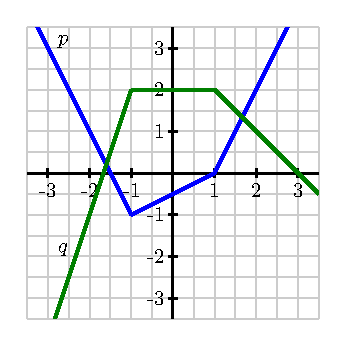
\includegraphics{figures/2_1_Ez3.eps}
\caption{The graphs of $p$ (in blue) and $q$ (in green).} \label{F:2.5.Ez3}
\end{center}
\end{figure}
\ba
	\item Let $C(x) = p(q(x))$.  Determine $C'(0)$ and $C'(3)$.
	\item Find a value of $x$ for which $C'(x)$ does not exist.  Explain your thinking.
	\item Let $Y(x) = q(q(x))$ and $Z(x) = q(p(x))$.  Determine $Y'(-2)$ and $Z'(0)$.	
\ea
\item If a spherical tank of radius 4 feet has $h$ feet of water present in the tank, then the volume of water in the tank is given by the formula
$$V = \frac{\pi}{3} h^2(12-h).$$
\ba
	\item At what instantaneous rate is the volume of water in the tank changing with respect to the \emph{height} of the water at the instant $h = 1$?  What are the units on this quantity?
	\item Now suppose that the height of water in the tank is being regulated by an inflow and outflow (e.g., a faucet and a drain) so that the height of the water at time $t$ is given by the rule $h(t) = \sin(\pi t) + 1$, where $t$ is measured in hours (and $h$ is still measured in feet).  At what rate is the height of the water changing with respect to time at the instant $t = 2$?
	\item Continuing under the assumptions in (b), at what instantaneous rate is the volume of water in the tank changing with respect to \emph{time} at the instant $t = 2$?  
	\item What are the main differences between the rates found in (a) and (c)?  Include a discussion of the relevant units.
\ea
\end{exercises}
\afterexercises